% Exact LaTeX recreation of the supplied Phase-1.pdf
% Compile with pdfLaTeX. Place member pictures in the same folder if required.

\documentclass[11pt,a4paper]{article}

\usepackage[a4paper,left=2.0cm,right=2.0cm,top=1.55cm,bottom=1.55cm]{geometry}
\usepackage[T1]{fontenc}
\usepackage{lmodern}
\usepackage{graphicx}
\usepackage{xcolor}
\usepackage{array}
\usepackage{tabularx}
\usepackage{ragged2e}
\usepackage{enumitem}
\usepackage{fancyhdr}
\usepackage{tikz}
\usepackage{setspace}

% -------------------------------------------------
% COLOURS
% -------------------------------------------------
\definecolor{TitleBlue}{RGB}{61,103,154}

% -------------------------------------------------
% GENERAL SETTINGS
% -------------------------------------------------
\setlength{\parindent}{0pt}
\setlength{\parskip}{0pt}
\renewcommand{\arraystretch}{1.0}

% The supplied document uses a clean sans-serif heading style
% and italic serif-style explanatory text.
\newcommand{\blueheading}[1]{%
    {\sffamily\color{TitleBlue}\fontsize{15}{18}\selectfont #1}%
}

\newcommand{\bluebigheading}[1]{%
    {\sffamily\bfseries\color{TitleBlue}\fontsize{16}{19}\selectfont #1}%
}

\newcommand{\instruction}[1]{%
    {\itshape\fontsize{10.5}{12.5}\selectfont #1}%
}

\newcommand{\answerbox}[2][3.0cm]{%
    \vspace{2pt}
    \noindent
    \fbox{%
        \begin{minipage}[t][#1][t]{\dimexpr\textwidth-2\fboxsep-2\fboxrule\relax}
            \vspace{1mm}
            \itshape #2
        \end{minipage}
    }
}

% -------------------------------------------------
% HEADER / FOOTER
% -------------------------------------------------
\pagestyle{fancy}
\fancyhf{}
\renewcommand{\headrulewidth}{0pt}
\renewcommand{\footrulewidth}{0pt}

\fancyhead[L]{%
    \sffamily\bfseries\itshape\fontsize{10.5}{12}\selectfont
    DSCPP-III-2026-T048 
}
\fancyhead[R]{%
    \sffamily\bfseries\fontsize{10.5}{12}\selectfont
    PROJECT PROPOSAL
}
\fancyfoot[R]{%
    \itshape\fontsize{10}{12}\selectfont
    Page \thepage
}
\setlength{\headheight}{14pt}
\setlength{\headsep}{23pt}
\setlength{\footskip}{24pt}

% -------------------------------------------------
% PAGE 1
% -------------------------------------------------
\begin{document}

\vspace*{4mm}

\bluebigheading{PROJECT AND TEAM INFORMATION}

\vspace{13mm}

\blueheading{Project Title}

\vspace{1mm}

\answerbox[1.0cm]{\textbf{MiniShell-Virtual Terminal} }

\vspace{13mm}

\blueheading{Student / Team Information}

\vspace{2mm}

% Team information table
% Compact 4-member layout so all members remain on Page 1.
\noindent
\begin{tabularx}{\textwidth}{|>{\RaggedRight\arraybackslash}p{0.69\textwidth}|>{\RaggedRight\arraybackslash}X|}
\hline
\begin{minipage}[t]{\linewidth}
\vspace{1.5mm}
\textit{Team Name:}\\[-1mm]

\vspace{1.5mm}
\end{minipage}
&
\begin{minipage}[t]{\linewidth}
\vspace{1.5mm}
\textit{Shell Builders}
\vspace{1.5mm}
\end{minipage}
\\
\hline
\begin{minipage}[t][3.25cm][t]{\linewidth}
\vspace{1.5mm}
\textbf{Team member 1 (Team Lead)}\\[-1mm]

\vspace{2.0cm}
\end{minipage}
&
\begin{minipage}[t][3.25cm][t]{\linewidth}
\vspace{1.5mm}
\textit{Ahuja,Mahak -- 2510010225 }\\
\textit{mehak.ahuja.agra@gmail.com}

\vspace{2mm}
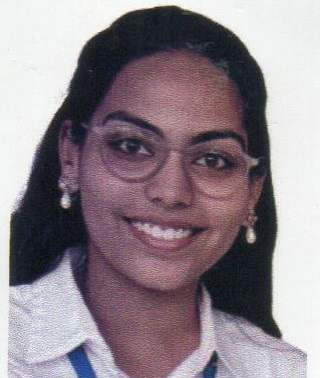
\includegraphics[width=3.0cm,height=1.5cm,keepaspectratio]{mahak.png}
\end{minipage}
\\
\hline
\begin{minipage}[t][3.25cm][t]{\linewidth}
\vspace{1.5mm}
\textbf{Team member 2}\\[-1mm]

\vspace{2.0cm}
\end{minipage}
&
\begin{minipage}[t][3.25cm][t]{\linewidth}
\vspace{1.5mm}
\textit{Jain, Anvi  -- \\ 2510350008}\\
\textit{anvijain026@gmail.com}

\vspace{2mm}
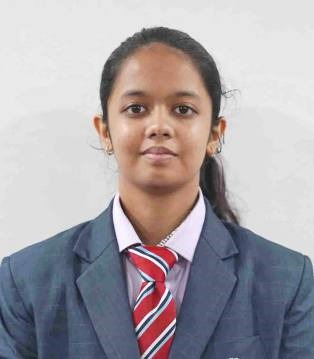
\includegraphics[width=3.0cm,height=1.5cm,keepaspectratio]{anvi.png}
\end{minipage}
\\
\hline
\begin{minipage}[t][3.25cm][t]{\linewidth}
\vspace{1.5mm}
\textbf{Team member 3}\\[-1mm]

\vspace{2.0cm}
\end{minipage}
&
\begin{minipage}[t][3.25cm][t]{\linewidth}
\vspace{1.5mm}
\textit{Bisht, Harshita -- 2510017763}\\
\textit{bharshita766@gmail.com}

\vspace{2mm}
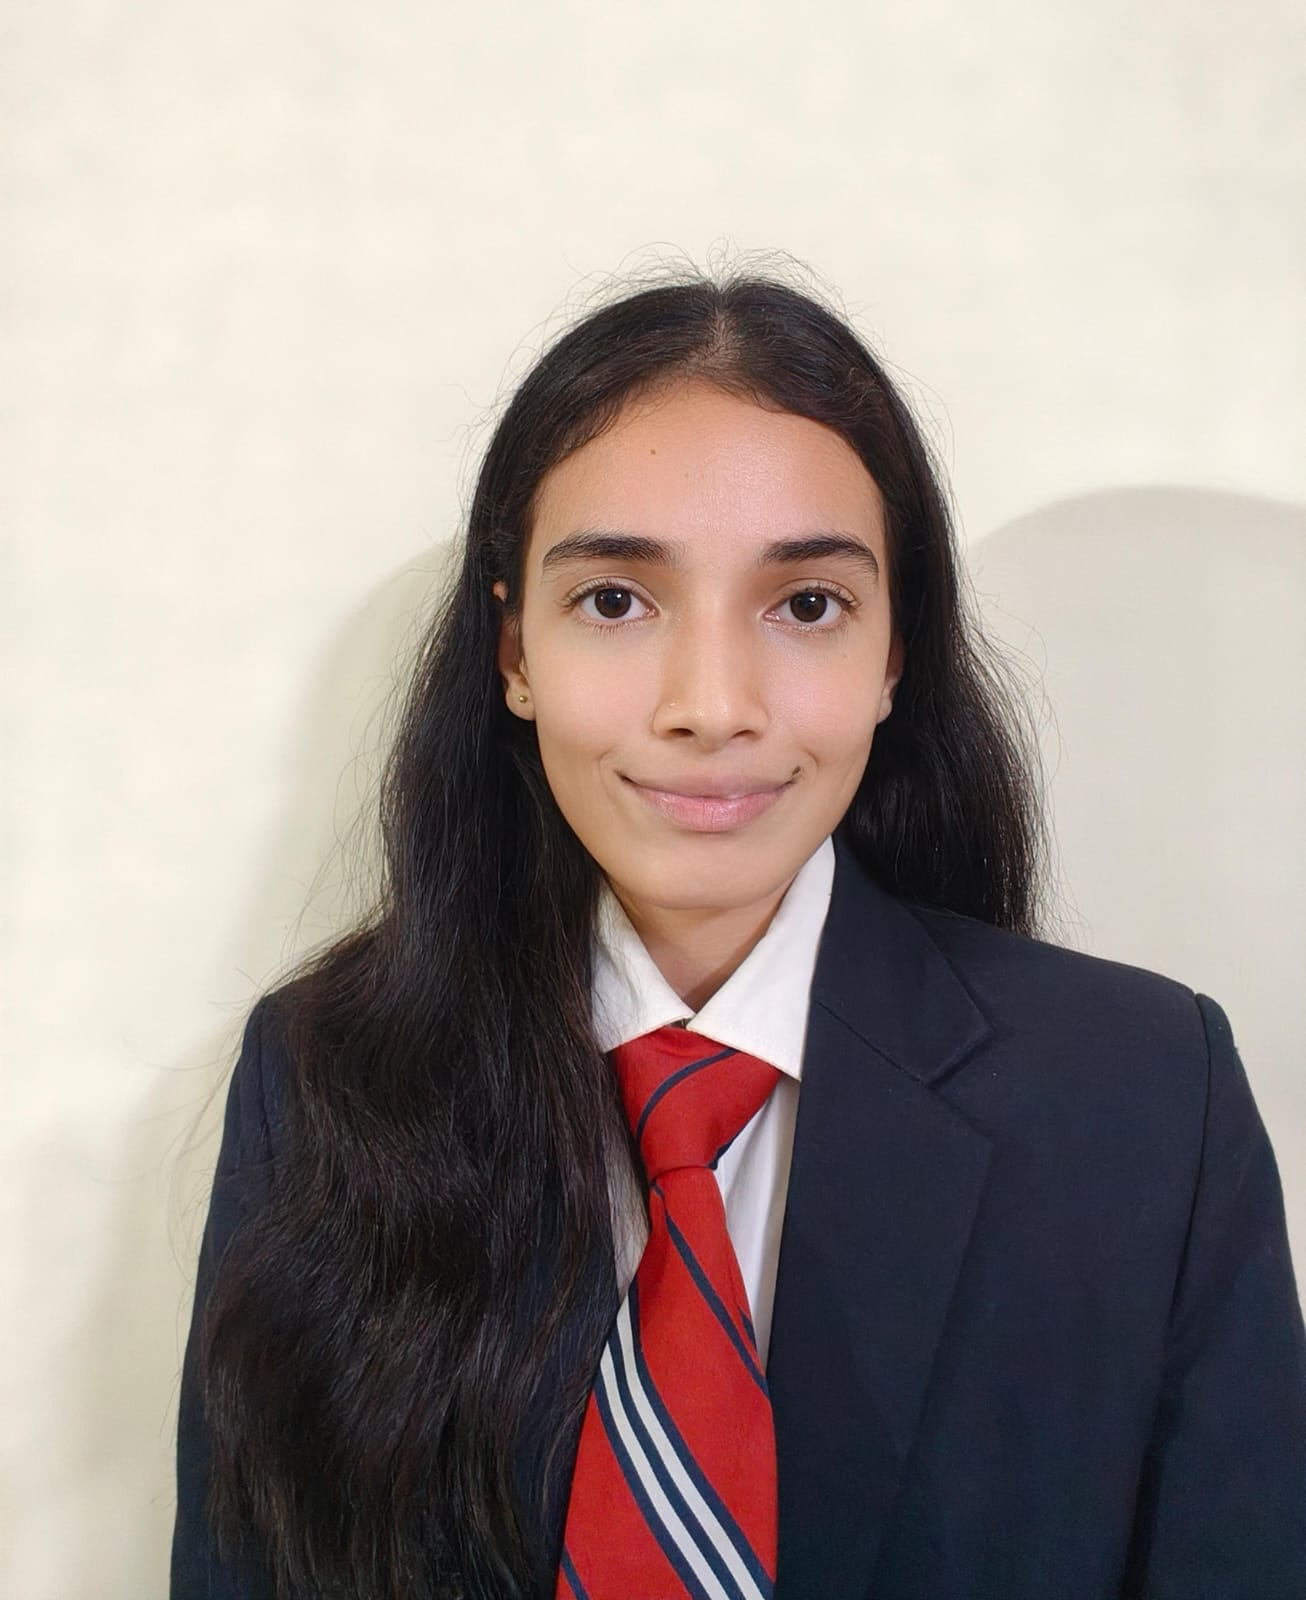
\includegraphics[width=3.0cm,height=1.5cm,keepaspectratio]{harshita.png}
\end{minipage}
\\
\hline
\begin{minipage}[t][3.25cm][t]{\linewidth}
\vspace{1.5mm}
\textbf{Team member 4}\\[-1mm]

\vspace{2.0cm}
\end{minipage}
&
\begin{minipage}[t][3.25cm][t]{\linewidth}
\vspace{1.5mm}
\textit{Jain , Samriddhi -- 2510370574}\\
\textit{email@example.com}

\vspace{2mm}
 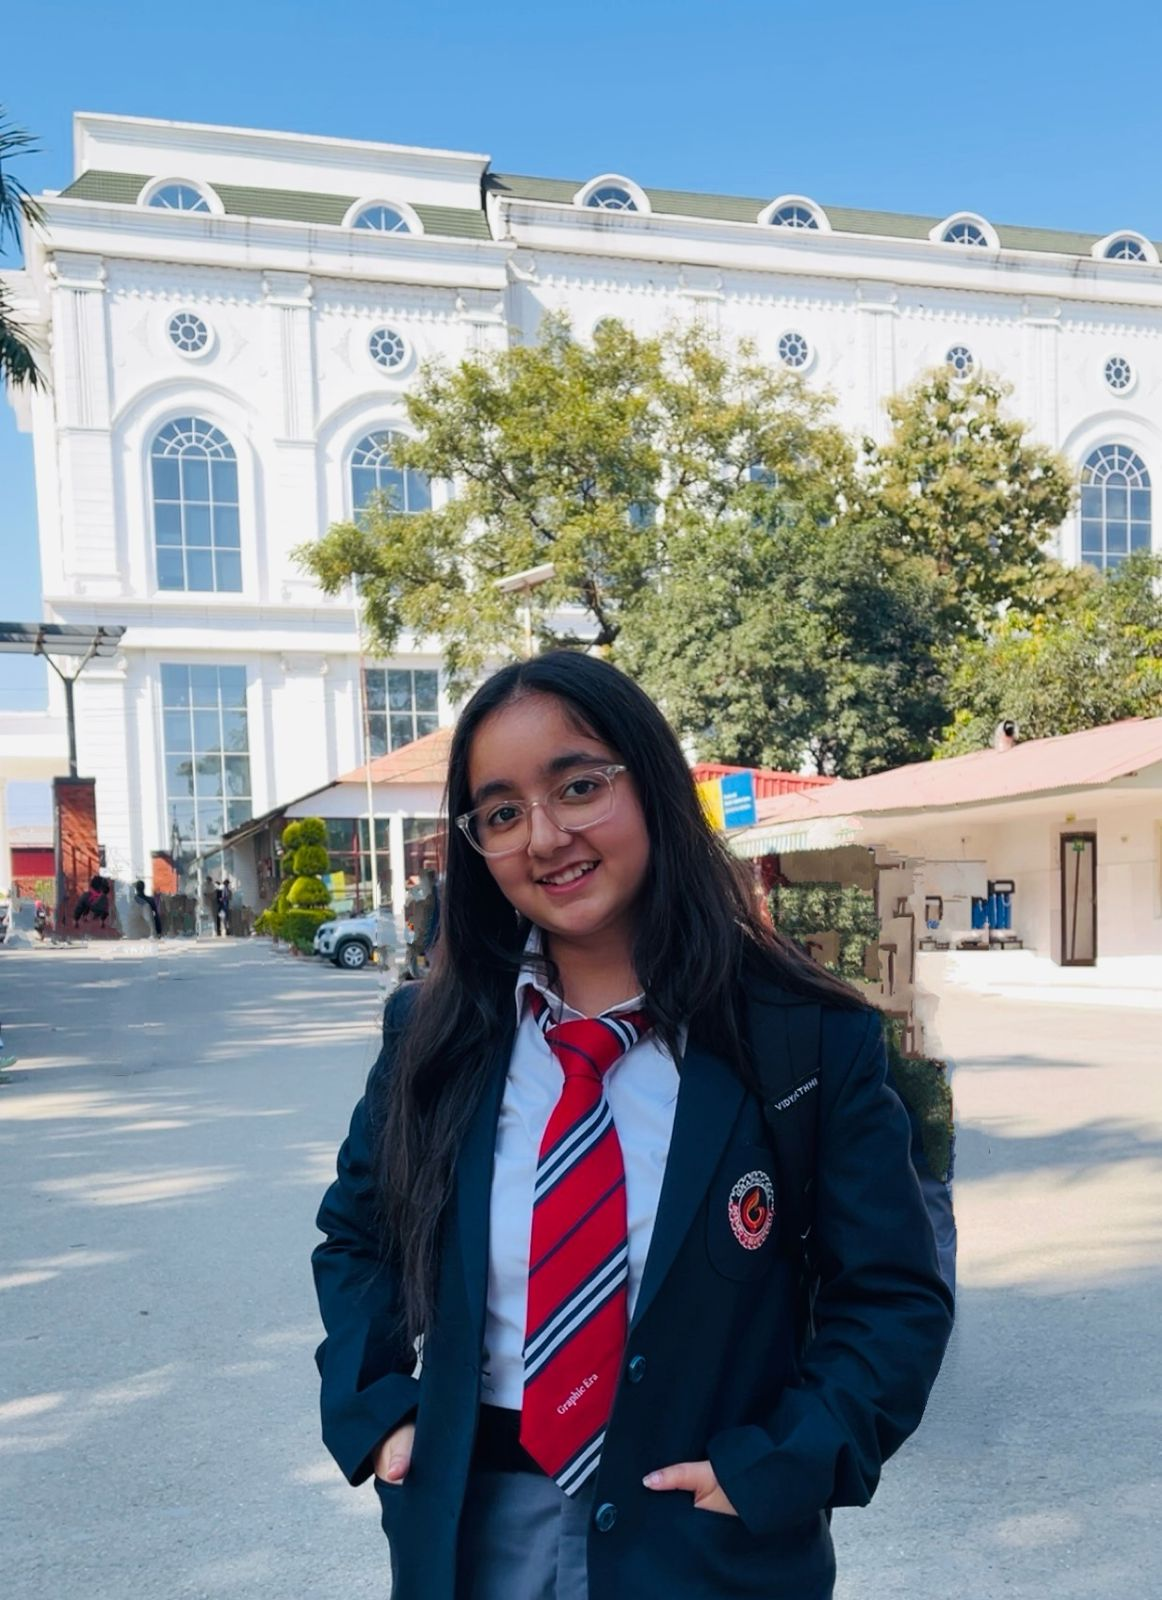
\includegraphics[width=3.0cm,height=1.5cm,keepaspectratio]{samriddhi.png}
\end{minipage}
\\
\hline
\end{tabularx}

\newpage

% -------------------------------------------------
% PAGE 2
% -------------------------------------------------

\bluebigheading{PROPOSAL DESCRIPTION (10 pts)}

\vspace{12mm}

\blueheading{Motivation (1 pt)}

\vspace{1mm}


\answerbox[10.0cm]{### Motivation

Understanding how an operating system manages files and how a command-line interface works internally can be quite challenging for beginners. Real file systems involve many complex concepts such as permissions, security, hardware interaction, and low-level operations, which can make them difficult to understand at an early stage. At the same time, students often study data structures like Trees, Stacks, and Hash Tables separately, without getting to see how these concepts can work together in a practical application.

This is where MiniShell – Virtual Terminal comes in. The main idea behind the project is to create a simple and safe environment where students can interact with a virtual file system using familiar shell commands. Instead of dealing with the complexity of a real operating system, users can explore concepts such as files, directories, paths, and navigation in a much easier way. This makes it easier to understand what actually happens behind the commands we use in a terminal.

Working on MiniShell also gives us an opportunity to apply the concepts we have learned in class to a practical, real-world-inspired problem. While developing the project, we make use of data structures, object-oriented programming, modular design, and command parsing, which helps strengthen both our programming and problem-solving skills.

Overall, MiniShell is more than just a basic terminal simulation. It is designed as a learning-oriented project that allows students to experiment with file-system concepts, understand how different data structures work together, and gain a better understanding of system-level programming in an interactive and beginner-friendly environment.
}

\vspace{12mm}

\blueheading{State of the Art / Current solution (1 pt)}

\vspace{1mm}

\answerbox[2.95cm]{Traditional operating systems like Linux, Unix, and Windows provide command-line tools that make it easy for users to work with files and folders. Using commands, users can create, delete, rename, search, and move between directories. However, the actual file systems behind these commands are much more complicated. They involve things like hardware, permissions, security, memory management, and other low-level operations. Because of this complexity, it can be difficult for beginners to understand what is really happening in the background when a simple command is executed.
}

\vspace{200mm}

\blueheading{Project Goals and Milestones (2 pts)}

\vspace{1mm}

\answerbox[19.0cm]{### Project Goals

The main aim of this project is to create a simple MiniShell using C++ that gives users a basic idea of how a command-line shell and file system work. The project will focus on:

\begin{itemize}
    \item  Creating a virtual file system using a Tree, where files and folders are organized in a hierarchy.

\item  Adding basic operations for creating, deleting, renaming, and managing files and directories.
\item  Using a Stack to keep track of the commands entered by the user.
\item Using a Hash Table to make searching for files and directories quicker.
\item Using important OOP concepts like encapsulation, inheritance, polymorphism, and abstraction while developing the system.
\item  Providing an interactive Command-Line Interface (CLI) through which users can enter commands and interact with the virtual file system.\end{itemize}

### Initial Milestones

We plan to develop the project in the following steps:

1. First, understand how basic terminals, shell commands, and file systems work.
2. Plan the structure of our virtual file system and decide how files and directories will be stored.
3. Build the Tree structure to represent the relationship between folders and files.
4. Add a Stack to store the history of commands entered by the user.
5. Implement a Hash Table to improve the speed of file and directory searches.
6. Create the required C++ classes and use OOP concepts to connect all the different parts of the project.

\textbf{OUR KEY FEATURES:\\
Menu display\\
Pop up while saving \\
Smart command correction\\}
\begin{itemize}
    \item MENU DISPLAY- In usual terminal commands are hard to be learnt by an amateur so we will provide a proper menu to the uers which conatins all the commands so no user faces issue.\\

\item Pop Up-While saving the document you dont have to select the path i.e desktop or documents in the menu bar ,rather a pop up will be shown so by no mistake it gets saved at wrong place.\\
\item Smart Command Correction-It is like an autocorect helping users and increses speed.
\end{itemize}
}

\vspace{100mm}

\blueheading{Project Approach (3 pts)}

\vspace{1mm}


\answerbox[10.0cm]{### 1. Virtual File System Design

We will create a simple virtual file system using a Tree data structure. In this structure, files and folders will be treated as nodes and connected in a way similar to a real file system. Users will be able to perform basic operations such as creating, deleting, renaming, navigating, and viewing files and folders through the shell.

### 2. DSA and OOP Implementation

The project will make use of important DSA concepts, mainly Trees, Stacks, and searching. These concepts will help us understand how different parts of the system work behind the commands entered by the user. The main application will be developed in C++ using OOP, with classes such as FSNode, File, Directory, FileSystem, and MiniShell. Concepts like encapsulation, inheritance, polymorphism, and abstraction will be used wherever they fit naturally into the design.

### 3. Technologies and Interface

The project will mainly use C and C++. C will be used for implementing and understanding the core DSA concepts, while C++ will be used to build the main application and apply OOP concepts. Users will interact with the system through a Command-Line Interface (CLI), where they can enter commands and perform different file-system operations. The project will be developed and tested using VS Code, and Git/GitHub may be used to keep track of the project and its changes.
}

\newpage

% -------------------------------------------------
% PAGE 3
% -------------------------------------------------

\blueheading{System Architecture (High Level Diagram)(2 pts)}

\vspace{1mm}


\answerbox[7.0cm]{%
    \centering
    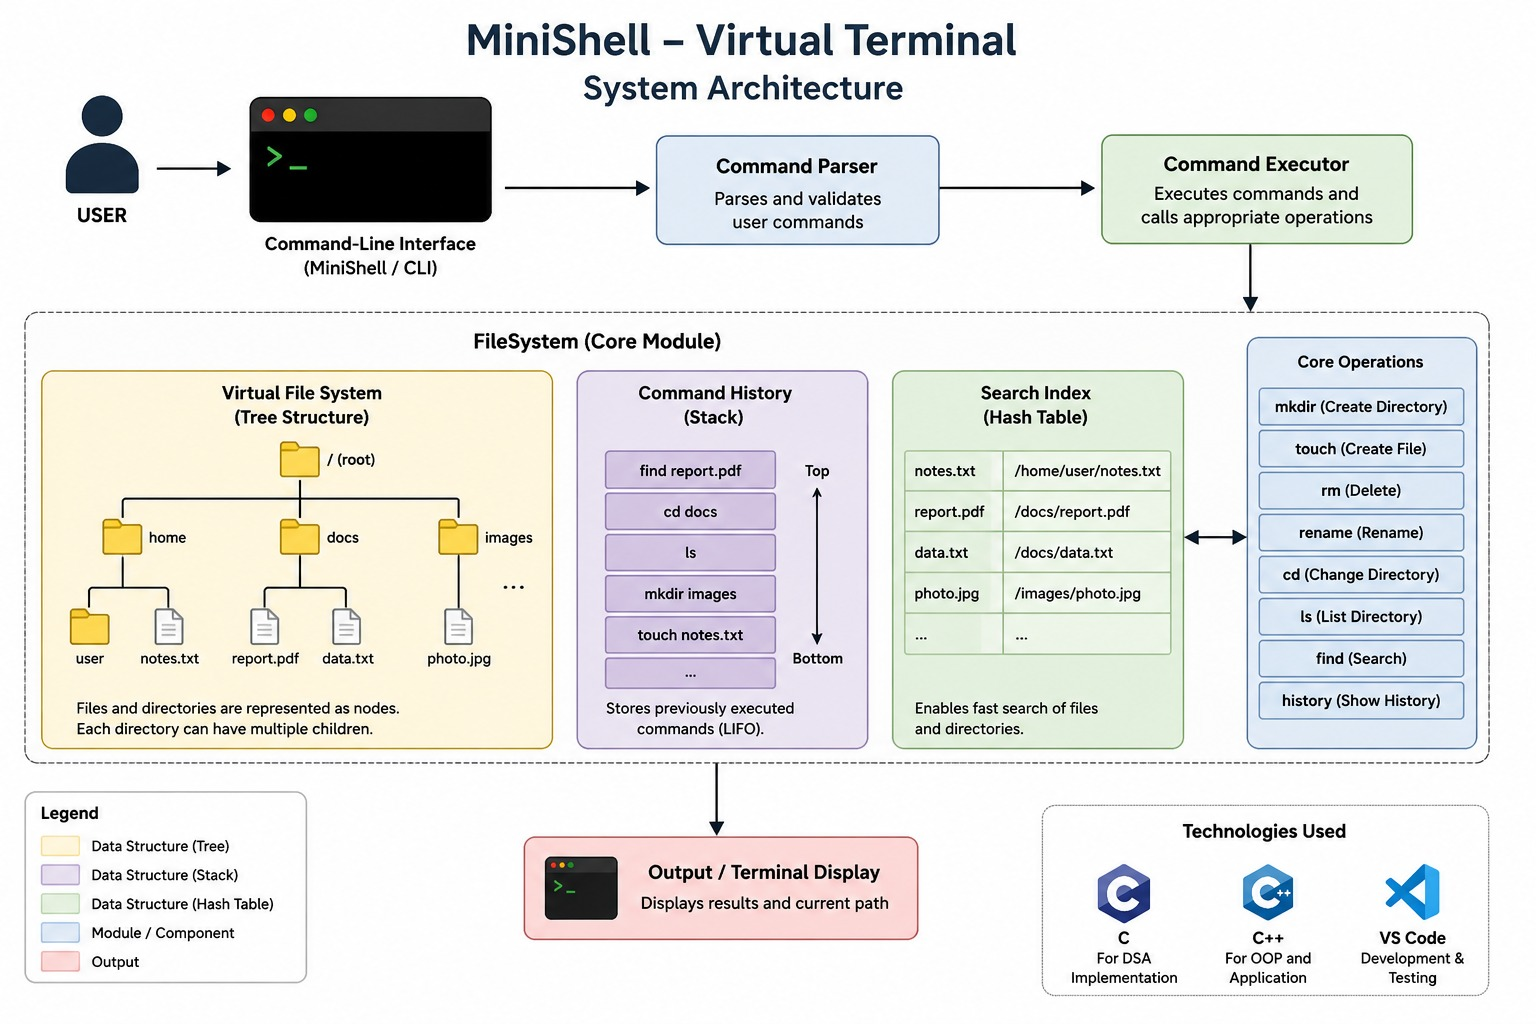
\includegraphics[
        width=2.0\linewidth,
        height=6.5cm,
        keepaspectratio
    ]{systemarchitecture.png}}

\vspace{12mm}

\blueheading{Project Outcome / Deliverables (1 pts)}

\vspace{1mm}

\answerbox[10.0cm]{### Expected Outcomes

By the end of the project, we aim to have a working Command-Line Interface through which users can interact with a virtual file system. The project will include:

\begin{itemize}
    \item - A hierarchical virtual file system for organizing files and folders.

\item - Basic operations such as creating, deleting, renaming, and navigating files and directories.
\item - The ability to search for files and folders.
\item - A command history feature using a Stack.
\item - A Hash Table to make searching more efficient.
\item - Practical implementation of Trees, Stacks, and searching techniques.
\item - Use of important OOP concepts in C++ while developing the system.
\end{itemize}

Overall, the project will provide a simple and interactive way to explore how basic terminal commands and file-system operations work behind the scenes, while also helping us apply the DSA and programming concepts we have learned in a practical project.
}

\vspace{200mm}

\blueheading{Assumptions}

\vspace{6mm}


\answerbox[7.0cm]{### Assumptions
 \begin{itemize}
     \item - We assume that the system will work as a virtual file system and will not make any changes to the user's actual files or folders.

\item - We assume that users will interact with the system through a Command-Line Interface (CLI).
\item -We assume that the system will support only the basic file-system commands required for the project, rather than all the commands available in a real operating system.
\item - We assume that the main purpose of the project is to understand and demonstrate DSA and OOP concepts, rather than to build a complete operating-system-level file system.
\item - We assume that the project will be developed and tested using C, C++, and VS Code.
 \end{itemize}

}

\vspace{12mm}

\blueheading{References}

\vspace{1mm}



\answerbox[5.0cm]{

\begin{enumerate}
    \item GeeksforGeeks – Data Structures and Algorithms

 \itemGeeksforGeeks – Tree Data Structure
\item GeeksforGeeks – Stack Data Structure
\item GeeksforGeeks – Hashing Data Structure
\item cppreference – C++ Language Reference
\item cppreference – C++ Standard Library
\item GNU Bash Reference Manual – Shell Concepts
\end{enumerate}

}
\end{document}
